% Preamble
\documentclass{article}


% Package Imports
\usepackage{../../../../mypackages}



% Macros
\usepackage{../../../../mymacros}


% Homework Details and Basic Document Settings
\pagestyle{fancy}
\lhead{\textbf{Eric Xia}}
\chead{MATH134 (Professor Ebru Bekyel): Week 3 Assignment}
\cfoot{\thepage}

\renewcommand\headrulewidth{0.4pt}
\renewcommand\footrulewidth{0.4pt}


% Title Page
\title{
    \vspace{2in}
    \textmd{\textbf{MATH134: Week 3 Assignment}}\\
    \normalsize\vspace{0.1in}\small{Due on October 19, 2020 at 5:45 PM}\\
    \vspace{0.1in}\large{\textit{Professor Ebru Bekyel}}
    \vspace{3in}
}

\author{\textbf{Eric Xia}}
\date{}


% Problem Headers and Footers
\fancypagestyle{page2}{\rhead{Section 3.1 Problem 57}\fancyfoot[L]{Section 3.1 Problem 59 continued on next page\ldots}}
\fancypagestyle{page3}{\rhead{Section 3.1 Problem 59}}
\fancypagestyle{page4}{\rhead{Section 3.2 Problem 50}\fancyfoot[L]{Section 3.2 Problem 62 continued on next page\ldots}}
\fancypagestyle{page5}{\rhead{Section 3.2 Problem 62}\fancyfoot[L]{Section 3.3 Problem 54 continued on next page\ldots}}
\fancypagestyle{page6}{\rhead{Section 3.3 Problem 54}\fancyfoot[L]{Section 3.3 Problem 54 continued on next page\ldots}}
\fancypagestyle{page7}{\rhead{Section 3.3 Problem 54}}
\fancypagestyle{page8}{\rhead{Section 3.5 Problem 62}\fancyfoot[L]{Section 3.6 Problem 67 continued on next page\ldots}}
\fancypagestyle{page9}{\rhead{Section 3.6 Problem 67}\fancyfoot[L]{Section 3.6 Problem 72 continued on next page\ldots}}
\fancypagestyle{page10}{\rhead{Section 3.6 Problem 72}\fancyfoot[L]{Section 3.7 Problem 52 continued on next page\ldots}}
\fancypagestyle{page11}{\rhead{Section 3.7 Problem 52}\fancyfoot[L]{Section 3.7 Problem 55 continued on next page\ldots}}
\fancypagestyle{page12}{\rhead{Section 3.7 Problem 55}}
\fancypagestyle{page13}{\rhead{Section 3.7 Problem 58}\fancyfoot[L]{Section 3.7 Problem 58 continued on next page\ldots}}
\fancypagestyle{page14}{\rhead{Section 3.7 Problem 58}}


%-------------------------------------------------------------------------------------------------------------------------------------------------------------------------------------------------------------------------
%-------------------------------------------------------------------------------------------------------------------------------------------------------------------------------------------------------------------------
%-------------------------------------------------------------------------------------------------------------------------------------------------------------------------------------------------------------------------
\begin{document}

    \maketitle
    \pagebreak


    \thispagestyle{page2}

    \begin{tbhtheorem}{Section 3.1 Problem 57}
        The lines tangent and normal to the graph of the squaring function at the point (3,9) intersect the $x$-axis at points $s$ units apart. What is $s$?
    \end{tbhtheorem}

    The slope of the squaring function at the point (3,9) is given by:

    \begin{align*}
        y  &= x^2 \\
        \frac{dy}{dx}\Big|_{x=3} &= 2(3) = 6
    \end{align*}

    Then the tangent and normal to the squaring function at the point (3,9) are:

    \begin{align*}
        y-9 &= 6(x-3)           & \text{ (Tangent)} \\
        y-9 &= -\frac{1}{6}(x-3)    & \text{ (Normal)}
    \end{align*}

    We can find the points at which the tangent and normal intersect the $x$-axis by setting $y=0$:

    \begin{align*}
        - 9 &= 6x - 18 \\
        x   &= \frac{3}{2} \implies \left(\frac{3}{2},0\right) \\
        -9  &= -\frac{1}{6}x + \frac{1}{2} \\
        x   &= 57 \implies (57,0)
    \end{align*}

    The distance, $s$, between these two points are:

    \[
        s = 57 - \frac{3}{2} = \frac{111}{2}
    \]



    \begin{tbhtheorem}{Section 3.1 Problem 59}
        Let
        \[
            f(x) =
            \begin{cases}
                x\sin{(\frac{1}{x})},   & x \not = 0 \\
                0,                      & x = 0
            \end{cases}
        \]
        and
        \[
            g(x) = xf(x)
        \]

        The graphs of $f$ and $g$ are indicated in the figures below:

        (a) Show that $f$ and $g$ are both continuous at 0. \\
        (b) Show that $f$ is not differentiable at 0. \\
        (c) Show that $g$ is differentiable at 0 and give $g'(0)$.
    \end{tbhtheorem}


    \begin{figure*}[hbt!]
        \centering
        \includegraphics[]{Homework3_Fig1.png}
    \end{figure*}

    \pagebreak
    \thispagestyle{page3}



    (a)
    \begin{proof}
        It is known that

        \[
            -1 \leq \sin{\left(\frac{1}{x}\right)} \leq 1
        \]

        Then it must be true that

        \[
            -x \leq x\sin{\left(\frac{1}{x}\right)} \leq x.
        \]

        Because

        \[
            \lim_{x\to 0} (-x) = \lim_{x\to 0} (x) = 0,
        \]

        then by the Squeeze Theorem, it is also true that

        \[
            \lim_{x\to 0} x\sin{\left(\frac{1}{x}\right)} = 0.
        \]

        Since this limit exists, by the definition of continuity, $f(x)$ is continuous at 0. \\

        The function $y=x$ is continuous for all $x$, including 0. Since $g(x)=xf(x)$ and both $x$ and $f(x)$ are continuous at 0, $g(x)$ must also be continuous at 0 by the definition of a function.
    \end{proof}

    (b)
    \begin{proof}
        If $f'(0)$ exists, then it is given by:

        \[
            \lim_{h\to 0} \frac{f(x+h)-f(x)}{h} = \lim_{h\to 0} \frac{f(h) - f(0)}{h}
        \]

        When $h=0$,

        \[
            \lim_{h\to 0} \frac{f(h) - f(0)}{h} = \lim_{h\to 0} \frac{0}{0}
        \]

       and the limit is undefined. When $h\not = 0$,

        \begin{align*}
            \lim_{h\to 0} \frac{f(h) - f(0)}{h} &= \lim_{h\to 0} \frac{\cancel{h}\sin{\left(\frac{1}{h}\right)}}{h} \\
                                                &= \lim_{h\to 0} \sin{\left(\frac{1}{h}\right)} \\
                                                &= \lim_{h\to 0} \sin{\left(\frac{1}{0}\right)}
        \end{align*}

       and the limit does not exist. Since

        \[
            \lim_{h\to 0} \frac{f(x+h)-f(x)}{h}, x = 0
        \]

        does not exist, hence by the definition of differentiability, $f$ is not differentiable at 0.
    \end{proof}

    (c)
    \begin{proof}
        By the definition of $g(x)$ as $g(x)=xf(x)$, $g(x)$ can be redefined as

        \[
            g(x) =
            \begin{cases}
                x^2 \sin{\left(\frac{1}{x}\right)}, & x \not = 0 \\
                0,                                  & x = 0
            \end{cases}
        \]

        Suppose that $g'(0)$ can be written as

        \begin{align*}
            g'(x) &= \lim_{h\to 0} \frac{g(x+h)-g(x)}{h} \\
            g'(0) &= \lim_{h\to 0} \frac{g(h) - g(0)}{h} \\
                  &= \lim_{h\to 0} \frac{h^2 \sin{\left(\frac{1}{h}\right)}}{h} \\
                  &= \lim_{h\to 0} h\sin{\left(\frac{1}{h}\right)} \\
                  &= 0
        \end{align*}

        Since the limit above exists, hence by the definition of the derivative, $g'(0)$ also exists and $g'(0)=0$.
    \end{proof}

    \pagebreak
    \thispagestyle{page4}


    \begin{tbhtheorem}{Section 3.2 Problem 50}
        Find $A$ and $B$ given that the derivative of

        \[
            f(x) =
            \begin{cases}
                Ax^2 + B,   & x < -1 \\
                Bx^5 + Ax + 4, & x \geq -1
            \end{cases}
        \]

        is everywhere continuous.
    \end{tbhtheorem}

    \begin{proof}
        Assume that $A$ and $B$ are constants. Because $f'(x)$ is continuous everywhere, including at 0,

        \[
            f'(x)   =
            \begin{cases}
                2Ax,        & x < -1 \\
                5Bx^4 + A,  & x \geq -1
            \end{cases}
        \]

        and

        \begin{align*}
            \lim_{x\to -1} 2Ax      &= 5B(-1)^4 + A \\
            -2A                     &= 5B + A \\
            -3A                     &= 5B \\
            A                       &= -\frac{5B}{3}.
        \end{align*}

        Since $f'(x)$ is continuous everywhere, it must be true that $f(x)$ has a derivative for every $x$ in its domain. Because differentiability, by definition, implies continuity, then $f(x)$ must be continuous along
        its entire domain, including at -1. Then it must be true that:

        \begin{align*}
            \lim_{x\to -1} Ax^2 + B &= B(-1)^5 + A(-1) + 4 \\
            A + B                   &= -B-A+4 \\
            4                       &= 2A + 2B \\
            A + B                   &= 2
        \end{align*}

        Because

        \[
            A = - \frac{5B}{3},
        \]

        $A+B=2$ can be rewritten as

        \begin{align*}
            - \frac{5B}{3} + B &= 2 \\
            - \frac{5B}{3} + \frac{3B}{3} &= 2 \\
            -\frac{2B}{3}                 &= 2 \\
            B                             &= -3
        \end{align*}

        Then the value of $A$ is given by:

        \[
            A = -\frac{5(-3)}{3} = 5
        \]

        Thus, $A = 5$ and $B=-3$.
    \end{proof}



    \begin{tbhtheorem}{Section 3.2 Problem 62}
        Set $f(x) = x^3$. \\
        (a) Find an equation for the line tangent to the graph of $f$ at $(c, f(c)), c\not = 0$. \\
        (b) Deteremine whether the tangent line found in (a) intersects the graph of $f$ at a point other than $(c,c^3)$. \\
        If it does, find the $x$-coordinate of the second point of intersection.
    \end{tbhtheorem}

    (a) \\
    When $x=c$,

    \begin{align*}
        \frac{dy}{dx}\Big|_{x=c} = 3c^2
    \end{align*}

    Let $y=f(x)$. Because $f(c)=c^3$, an equation for the line tangent to the graph of $f$ at $(c,c^3),c\not = 0$ is:

    \[
        y-c^3 = 3c^2 (x-c).
    \]

    \pagebreak
    \thispagestyle{page5}

    (b) \\
    Let $y=f(x)$. If the tangent line found in (a) intersects the graph of $f$ at a point other than $(c,c^3)$, then these points are found by solving $(x,y)$ for the system below:

    \begin{align*}
        \begin{cases}
            y = x^3     & (1)\\
            y - c^3 = 3c^2 (x-c) & (2)
        \end{cases}
    \end{align*}

    Substituting $y=x^3$ into equation (2), the equation becomes

    \begin{align*}
        x^3 - c^3   &= 3c^2 (x-c) \\
        \frac{(x-c)(x^2 + xc + c^2)}{x-c}   &= 3c^2 (x-c) \\
        x^2 + xc + c^2                      &= 3c^2 \\
        x^2 + xc -2c^2                      &= 0 \\
        x^2 - xc + 2xc -2c^2                &= 0 \\
        x(x-c) + 2c(x-c)                    &= 0 \\
        (x-c)(x+2c)                         &= 0 \\
        x                                   &= -2c, c
    \end{align*}

    Thus, the $x$-coordinate of the other point of intersection is $x=-2c$. \\



    \begin{tbhtheorem}{Section 3.3 Problem 54}
        Set
        \[
            g(x) =
            \begin{cases}
                x^3,    & x \geq 0 \\
                0,      & x < 0.
            \end{cases}
        \]
        (a) Find $g'(0)$ and $g"(0)$. \\
        (b) Determine $g'(x)$ and $g"(x)$ for all other $x$. \\
        (c) Show that $g'''(0)$ does not exist. \\
        (d) Sketch the graphs of $g, g', g"$.
    \end{tbhtheorem}


    (a-b) \\
    If $g'(0)$ exists, then by the definition of a derivative, it is given by:

    \begin{align*}
        g'(0)   &= \lim_{x\to 0} \frac{g(x) - g(0)}{x}
    \end{align*}

    For $x<0$,

    \begin{align*}
        \lim_{x\to 0^-} \frac{g(x) - g(0)}{x}   &= \lim_{x\to 0} \frac{-x^3}{x} \\
                                                &= \lim_{x\to 0} -x^2 \\
                                                &= 0
    \end{align*}

    For $x>0$,

    \begin{align*}
        \lim_{x\to 0^+} \frac{g(x) - g(0)}{x}   &= \lim_{x\to 0} \frac{x^3 - x^3}{x} \\
                                                &= \lim_{x\to 0}x^2 - x^2 \\
                                                &= 0
    \end{align*}

    Thus, $g(x)$ is differentiable at 0 and

    \[
        g'(0) = 0.
    \]

    The derivatives of the pieces of the piecewise function $g(x)$ are given by:

    \begin{align*}
        \frac{d}{dx} x^3 &= 3x^2 \\
        \frac{d}{dx} 0   &= 0
    \end{align*}

    Because $\frac{d}{dx}\Big|_{x=0} x^3 = 3(0)^2 = 0$ aligns with the limit-computed value of $g'(0)=0$, then it suffices to write that $g'(x)$ can be defined as:

    \[
        g'(x)   =
        \begin{cases}
            3x^2,   & x \geq 0 \\
            0,      & x < 0
        \end{cases}
    \]

    \pagebreak
    \thispagestyle{page6}

    If $g"(0)$ exists, then it is given by:

    \[
        g"(0) = \lim_{x\to 0} \frac{g'(x) - g'(0)}{x}
    \]

    For $x<0$,

    \begin{align*}
        \lim_{x\to 0^-} \frac{g'(x) - g'(0)}{x}     &= \lim_{x\to 0} \frac{-3x^2}{x} \\
                                                    &= \lim_{x\to 0} -3x \\
                                                    &= 0
    \end{align*}

    For $x>0$,

    \begin{align*}
        \lim_{x\to 0^+} \frac{g'(x) - g'(0)}{x}     &= \lim_{x\to 0} \frac{3x^2 - 3x^2}{x} \\
                                                    &= \lim_{x\to 0} 3x - 3x \\
                                                    &= 0
    \end{align*}

    Thus, $g'(x)$ is differentiable at 0 and

    \[
        g"(0) = 0.
    \]

    The derivatives of the pieces of the piecewise function $g'(x)$ are given by:

    \begin{align*}
        \frac{d}{dx} 3x^2 &= 6x \\
        \frac{d}{dx} 0    &= 0
    \end{align*}

    Because $\frac{d}{dx}\Big|_{x=0} 3x^2 = 3(0)^2 = 0$ aligns with the limit-computed value of $g"(0)=0$, then it suffices to write that $g"(x)$ can be defined as:

    \[
        g"(x) =
        \begin{cases}
            6x, & x \geq 0 \\
            0,  & x < 0
        \end{cases}
    \]

    (c) \\

    If $g'''(0)$ exists, then by the definition of the derivative, it is given by:

    \[
       \lim_{x\to 0} \frac{g"(x) - g"(0)}{x} = 6(0) = 0
    \]

    For $x < 0$,

    \begin{align*}
        \lim_{x\to 0^-} \frac{g"(x) - g"(0)}{x} &= \lim_{x\to 0} \frac{-6x}{x} \\
                                                &= -6
    \end{align*}

    For $x>0$,

    \begin{align*}
        \lim_{x\to 0^+} \frac{g"(x) - g"(0)}{x} &= \lim_{x\to 0} \frac{6x-6x}{x} \\
                                                &= \lim_{x\to 0} 6 - 6 \\
                                                &= 0
    \end{align*}

    Because

    \[
        \lim_{x\to 0^-} \frac{g"(x) - g"(0)}{x} \not = \lim_{x\to 0^+} \frac{g"(x) - g"(0)}{x},
    \]

    by the definition of the derivative, $g'''(0)$ does not exist.

    \pagebreak
    \thispagestyle{page7}

    (d)

    \begin{center}
        \begin{tabular}{ccc}
            \begin{tikzpicture}[scale=0.75]
                \begin{axis}[
                axis lines = center,
                axis equal image,
                xmin = -5,
                xmax = 5,
                ymin = -2,
                ymax = 12
                ]
                    \addplot[
                    color = blue,
                    domain = 0:5
                    ]
                    {x^3};
                    \addlegendentry{$g(x)$}
                    \addplot[
                    color = blue,
                    domain = -5:0
                    ]
                    {0};
                \end{axis}
            \end{tikzpicture}
            %
            &
            %
            \begin{tikzpicture}[scale=0.75]
                \begin{axis}[
                axis lines = center,
                axis equal image,
                xmin = -5,
                xmax = 5,
                ymin = -2,
                ymax = 12
                ]
                    \addplot[
                    color = blue,
                    domain = 0:5
                    ]
                    {3*x^2};
                    \addlegendentry{$g'(x)$}
                    \addplot[
                    color = blue,
                    domain = -5:0
                    ]
                    {0};
                \end{axis}
            \end{tikzpicture}
            %
            &
            %
            \begin{tikzpicture}[scale=0.75]
                \begin{axis}[
                axis lines = center,
                axis equal image,
                xmin = -5,
                xmax = 5,
                ymin = -2,
                ymax = 12
                ]
                    \addplot[
                    color = blue,
                    domain = 0:5
                    ]
                    {6*x};
                    \addlegendentry{$g"(x)$}
                    \addplot[
                    color = blue,
                    domain = -5:0
                    ]
                    {0};
                \end{axis}
            \end{tikzpicture}
        \end{tabular}
    \end{center}




    \begin{tbhtheorem}{Section 3.3 Problem 72}
        Set
        \[
            f(x) = \frac{1}{2}x^3 - 3x^2 + 4x + 1.
        \]

        (a) Calculate $f'(x)$ \\
        (b) Use a graphing utility to display in one figure the graphs of $f$ and $f'$. If possible, graph $f$ and $f'$ in different colors. \\
        (c) What can you say about the graph of $f$ where $f'(x)=0$? \\
        (d) Find the $x$-coordinate of each point where the tangent to the graph of $f$ is horizontal by finding the zeros of $f'$ to three decimal places.
    \end{tbhtheorem}

    (a)

    \[
        f'(x) = \frac{3}{2}x^2 - 6x + 4
    \]

    (b)

    \begin{center}
        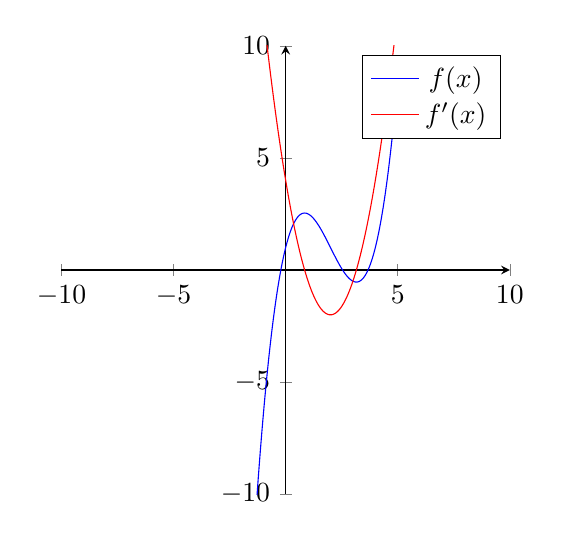
\begin{tikzpicture}[scale= 1]
            \begin{axis}[
                axis lines = center,
                axis equal image,
                xmin = -10,
                xmax = 10,
                ymin = -10,
                ymax = 10,
            ]
            \addplot[
                color = blue,
                samples = 300
            ]
            {0.5*x^3-3*x^2+4*x+1};
            \addlegendentry{$f(x)$}
            \addplot[
                color = red,
                samples = 300
            ]
            {1.5*x^2-6*x+4};
            \addlegendentry{$f'(x)$}
            \end{axis}
        \end{tikzpicture}
    \end{center}

    (c) \\
    At the points where $f'(x)=0$, the graph of $f(x)$ reaches its relative extrema and has a slope of 0. \\

    (d) \\
    When $f'(x)=0$,

    \begin{align*}
        \frac{3}{2}x^2 - 6x + 4 &= 0 \\
        3x^2 - 12x + 8          &= 0 \\
        x                       &= \frac{12\pm \sqrt{(-12)^2 - 4(3)(8)}}{2(3)} \\
        x                       &= 0.845, 3.155
    \end{align*}

    Hence, the $x$-coordinates of the points where the tangents to the graph of $f$ are horizontal are $x=0.845,3.155$

    \pagebreak
    \thispagestyle{page8}

    \begin{tbhtheorem}{Section 3.5 Problem 62}
        Let $f$ be a differentiable function. Use the chain rule to show that: \\
        (a) if $f$ is even, then $f'$ is odd. \\
        (b) if $f$ is odd, then $f'$ is even.
    \end{tbhtheorem}

    (a)

    \begin{proof}
        Let $f$ be a function of $x$. Because $f(x)$ is even,

        \[
            f(-x) = f(x).
        \]

        Then,

        \begin{align*}
            \frac{d}{dx} f(-x)  &= \frac{d}{dx} f(x) \\
            f'(-x) \cdot -1     &= f'(x) \cdot 1 \\
            -f'(-x)             &= f'(x) \\
            f'(-x)              &= -f'(x)
        \end{align*}

        Hence, by the definition of a function, $f'(x)$ is odd.
    \end{proof}

    (b)



    \begin{proof}
        Let $f$ be a function of $x$. Because $f(x)$ is odd,

        \[
            f(-x) = -f(x).
        \]

        Then,

        \begin{align*}
            \frac{d}{dx} f(-x)  &= -\frac{d}{dx} f(x) \\
            f'(-x) \cdot -1     &= -f'(x) \cdot 1 \\
            -f'(-x)             &= -f'(x) \\
            f'(-x)              &= f'(x)
        \end{align*}

        Hence, by the definition of a function, $f'(x)$ is even.
    \end{proof}


    \begin{tbhtheorem}{Section 3.6 Problem 67}
        Set
        \[
            f(x) =
            \begin{cases}
                x\sin{\left(\frac{1}{x}\right)},    & x\not = 0 \\
                0,                                  & x = 0
            \end{cases}
        \]

        and

        \[
            g(x) = xf(x).
        \]

        In Exercise 62, Section 3.1, you were asked to show that $f$ is continuous at 0 but not differentiable there, and that $g$ is differentiable at 0. Both $f$ and $g$ are differentiable at each $x\not = 0$. \\
        (a) Find $f'(x)$ and $g'(x)$ for $x\not = 0$. \\
        (b) Show that $g'$ is not continuous at 0.
    \end{tbhtheorem}

    (a) \\
    It is given that $f$ is differentiable for $x\not = 0$. When $x\not = 0$, $f(x) = x\sin{\left(\frac{1}{x}\right)}$. Then,

    \begin{align*}
        f'(x)       &= \sin{\left(\frac{1}{x}\right)} + x\cos{\left(\frac{1}{x}\right)} \cdot -\frac{1}{x^2}, x\not = 0 \\
                    &= \sin{\left(\frac{1}{x}\right)} - \frac{\cos{\left(\frac{1}{x}\right)}}{x}, x\not = 0
    \end{align*}

    Similarly, it is given that $g$ is differentiable for $x\not = 0$. When $x\not = 0$, $g(x) = x^2 \sin{\left(\frac{1}{x}\right)}$. Then,

    \begin{align*}
        g'(x)       &= 2x\sin{\left(\frac{1}{x}\right)} + x^2 \cos{\left(\frac{1}{x}\right)} \cdot -\frac{1}{x^2}, x\not = 0 \\
                    &= 2x\sin{\left(\frac{1}{x}\right)} - \cos{\left(\frac{1}{x}\right)}, x\not = 0
    \end{align*}

    \pagebreak
    \thispagestyle{page9}

    (b)
    \begin{proof}
        Suppose that $g'(x)$ is continuous at 0. Then by the definition of continuity, $\lim_{x\to 0} g'(x)$ exists. Because

        \[
            x\to 0 \implies x\not = 0,
        \]

        the limit becomes

        \begin{align*}
            \lim_{x\to 0} g'(x) &= \lim_{x\to 0} 2x\sin{\left(\frac{1}{x}\right)} - \cos{\left(\frac{1}{x}\right)} \\
            &= -\lim_{x\to 0} \cos{\left(\frac{1}{x}\right)} \\
            &= -\cos{\left(\frac{1}{0}\right)}.
        \end{align*}

        This limit does not exist and the assumption that $g'(x)$ is continuous at 0 has led to a contradiction. We can conclude therefore that $g'(x)$ \textit{is not} continuous at 0.
    \end{proof}




    \begin{tbhtheorem}{Section 3.6 Problem 72}
        A simple pendulum consists of a mass $m$ swinging at the end of a rod or wire of negligible mass. The figure shows a simple pendulum of length $L$. The angular displacement $\theta$ at time $t$ is given by a
        trigonometric expression:

        \[
            \theta (t) = A\sin{(\omega t + \phi)}
        \]

        where $A, \omega, \phi$ are constants. \\
        (a) Show that the function $\theta$ satisfies the equation
        \[
            \frac{d^2 \theta}{dt^2} + \omega ^2 \theta = 0.
        \]
        (Except for notation, this is the equation of Exercise 71.) \\
        (b) Show that $\theta$ can be written in the form

        \[
            \theta (t) = A\sin{(\omega t)} + B\cos{(\omega t)},
        \]

        where $A,B,\omega$ are constants.
    \end{tbhtheorem}

    \begin{figure*}[hbt!]
        \centering
        \includegraphics[]{Homework3_Fig2}
    \end{figure*}

    (a)


    Differentiating both sides of the definition of $\theta(t)$,

    \begin{align*}
        \frac{d\theta}{dt}  &= A\cos{(\omega t + \phi)}(w) = A\omega \cos{(\omega t + \phi)}
    \end{align*}

    and

    \begin{align*}
        \frac{d^2 \theta}{dt^2}                                     &= -A\omega\sin{(\omega t + \phi)}{\omega} \\
                                                                    &= -\omega ^2 A\sin{(\omega t + \phi)} \\
        \frac{d^2 \theta}{dt^2} + \omega ^2 A\sin{(\omega t + \phi)}  &= 0 \\
        \frac{d^2 \theta}{dt^2} + \omega ^2 \theta                  &= 0
    \end{align*}

    \pagebreak
    \thispagestyle{page10}

    (b)

    \begin{align*}
        \theta (t)  &= A\sin{(\omega t + \phi)} \\
                    &= A\sin{(\omega t)}\cos{(\phi)} + A\cos{(\omega t)}\sin{(\phi)}
    \end{align*}

    As $A$ and $B$ are constants, let them be redefined as:

    \[
        A = A\cos(\phi)
    \]

    and

    \[
        B = A\sin(\phi).
    \]

    Substituting these values of $A$ and $B$ into the earlier equation,

    \begin{align*}
        \theta(t)   &= A\sin{(\omega t)} + B\cos{(\omega t)}
    \end{align*}

    and hence $\theta(t)$ can be expressed in the above form.



    \begin{tbhtheorem}{Section 3.7 Problem 52 (Graph several of these)}
        Show that the family of parabolas $x = ay^2$ and the family of ellipses $x^2 + \frac{1}{2}y^2 = b$ are orthogonal trajectories of each other.
    \end{tbhtheorem}

    \begin{proof}
        The gradient at any point of the parabolic family $x=ay^2$ is given by:

        \begin{align*}
            \frac{d}{dx} x  &= a\frac{d}{dx} y^2 \\
            1               &= 2ay \frac{d}{dx} \\
            \frac{d}{dx}    &= \frac{1}{2ay}.
        \end{align*}

        The gradient at any point of the elliptical family $x^2 + \frac{1}{2} y^2 = b$ is given by:

        \begin{align*}
            \frac{d}{dx} x^2 + \frac{1}{2} \cdot \frac{d}{dx} y^2   &= \frac{d}{dx} b \\
            2x + y\frac{d}{dx}                                      &= 0 \\
            y\frac{d}{dx}                                           &= -2x \\
            \frac{d}{dx}                                            &= -\frac{2x}{y} \\
            \frac{d}{dx}                                            &= -\frac{2ay^2}{y} \\
            \frac{d}{dx}                                            &= -2ay
        \end{align*}

        The gradients $\frac{1}{2ay}$ and $-2ay$ are orthogonal for every $x$ and $y$, hence the family of parabolas $x=ay^2$ and the family of ellipses $x^2 + \frac{1}{2}y^2 = b$ are orthogonal trajectories of each
        other.
    \end{proof}

    Several examples demonstrating this orthogonal relationship are below, in which the blue curves are the parabolas the red curves are the ellipses. \\

    When $a=2$ and $b=3$,

    \begin{align*}
        x &= 2y^2 \\
        x^2 + \frac{1}{2} y^2 &= 3
    \end{align*}

    and the graph is:

    \begin{center}
        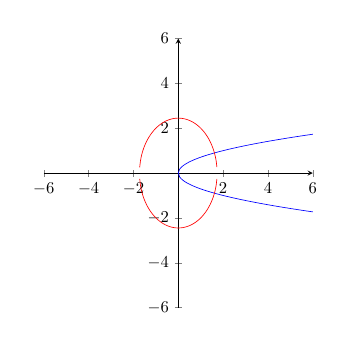
\begin{tikzpicture}[scale= 0.6]
            \begin{axis}[
                axis lines = center,
                axis equal image,
                xmin = -6,
                xmax = 6,
                ymin = -6,
                ymax = 6
            ]
            \addplot[
                samples = 100,
                color = blue,
                domain = 0:6
            ]
            {sqrt(x/2)};
            \addplot[
                samples = 100,
                color = blue,
                domain = 0:6
            ]
            {-sqrt(x/2)};
            \addplot[
                samples = 300,
                color = red,
                range = 0:2.449
            ]
            {sqrt(6-2*x^2)};
            \addplot[
                samples = 300,
                color = red,
                range = -2.449:0
            ]
            {-sqrt(6-2*x^2)};
            \end{axis}
        \end{tikzpicture}
    \end{center}

    \pagebreak
    \thispagestyle{page11}

    When $a=-3$ and $b=5$,

    \begin{align*}
        x                       &= -3y^2 \\
        x^2 + \frac{1}{2}y^2    &= 5
    \end{align*}

    and the graph is

    \begin{center}
        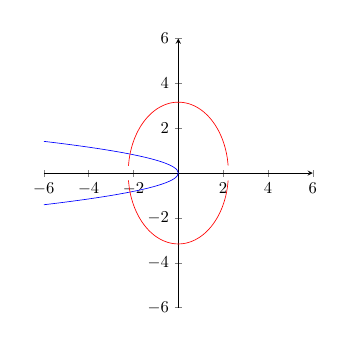
\begin{tikzpicture}[scale= 0.6]
            \begin{axis}[
                axis lines = center,
                axis equal image,
                xmin = -6,
                xmax = 6,
                ymin = -6,
                ymax = 6,
            ]
            \addplot[
                samples = 100,
                color = blue,
                domain = -6:0
            ]
            {sqrt(-x/3)};
            \addplot[
                samples = 100,
                color = blue,
                domain = -6:0
            ]
            {-sqrt(-x/3)};
            \addplot[
                samples = 300,
                color = red
            ]
            {sqrt(10-2*x^2)};
            \addplot[
                samples = 300,
                color = red
            ]
            {-sqrt(10-2*x^2)};
            \end{axis}
        \end{tikzpicture}
    \end{center}



    \begin{tbhtheorem}{Section 3.7 Problem 55}
        The curve

        \[
            (x^2 + y^2) ^2 = x^2 - y^2
        \]

        is called a lemniscate. The curve is shown in the figure. Find the four points of the curve at which the tangent line is horizontal.
    \end{tbhtheorem}

    \begin{figure*}[hbt!]
        \centering
        \includegraphics[]{Homework3_Fig3}
    \end{figure*}

    The tangent line is horizontal when the gradient of the curve is equal to 0. The gradient of the curve is given by:

    \begin{align*}
        \frac{d}{dx} (x^2+y^2)^2    &= \frac{d}{dx} (x^2-y^2) \\
        \frac{d}{dx} (x^4 + 2x^2 y^2 + y^4) &= 2x - 2yy' \\
        4x^3  + 4xy^2 + 4x^2 y y' + 4y^3 y' &= 2x - 2yy'
    \end{align*}

    When $y'=0$,

    \begin{align*}
        4x^3 + 4xy^2        &= 2x \\
        2x^3 + 2xy^2 - x    &= 0 \\
        x(2x^2 + 2y^2 -1)   &= 0
    \end{align*}

    When $x=0$,

    \begin{align*}
        (0+y^2)^2   &= 0 - y^2 \\
        y^4 + y^2   &= 0 \\
        y^2(y^2 + 1)    &= 0 \\
        y^2             &= 0, -1 \\
        y               &= 0, i, -i
    \end{align*}

    Because $x,y\in\mathbb{R}$ for the problem, when $x=0$, $y=0$. However, there is no solution at $(0,0)$ because the lemniscate is not differentiable at (0,0):

    \begin{align*}
        4(0)^3 + 4(0)(0)^2 + 4(0)^2(0) y' + 4(0)^3 y'   &= 2(0) - 2(0) y' \\
        0                                               &= 0
    \end{align*}

    \pagebreak
    \thispagestyle{page12}

    Hence, the points with horizontal tangent lines to the lemniscate are found by solving

    \[
        2x^2 + 2y^2 - 1 = 0
    \]

    The lemniscate is defined as

    \[
        (x^2+y^2)^2 = x^2 - y^2,
    \]

    so this equation can be rewritten as

    \begin{align*}
        2(x^2 + y^2) - 1    &= 0 \\
        2(\pm\sqrt{x^2 - y^2}) - 1  &= 0
    \end{align*}

    We now set up a system of equations to solve. Note that as we plan on removing the square root in the equation by re-squaring it, the negative case of the "$\pm\sqrt{x^2-y^2}$" can be safely ignored. Then,

    \[
        \begin{cases}
            2x^2 + 2y^2 - 1 = 0    & (1) \\
            2\sqrt{x^2 - y^2} = 0  & (2)
        \end{cases}
    \]

    Isolating $x^2$ for equation (1),

    \begin{align*}
        2x^2    &= 1-2y^2 \\
        x^2     &= \frac{1}{2} - y^2
    \end{align*}

    Then equation (2) can be rewritten and solved like so:

    \begin{align*}
        -2 \sqrt{\frac{1}{2}-y^2-y^2}-1    &= 0 \\
        \sqrt{\frac{1}{2}-2y^2}            &= \frac{1}{2} \\
        \frac{1}{2}-2y^2                   &= \frac{1}{4} \\
        -2y^2                              &= -\frac{1}{4} \\
        y^2                                &= \frac{1}{8} \\
        y                                  &= \pm \frac{\sqrt{1}}{\sqrt{8}} \cdot \frac{\sqrt{8}}{\sqrt{8}} \\
        y                                  &= \pm \frac{\sqrt{2}}{4}
    \end{align*}

    Returning to the $x$-isolated form of equation (1),

    \begin{align*}
        x^2 &= \frac{1}{2} - \left(\frac{\sqrt{2}}{4}\right) \\
        x   &= \pm \frac{\sqrt{6}}{4}
    \end{align*}

    and

    \[
        x^2 &= \frac{1}{2} - \left(-\frac{\sqrt{2}}{4}\right) \\
        x   &= \pm \frac{\sqrt{6}}{4}
    \]

    Thus, the four points of the curve at which the tangent line is horizontal are:

    \[
        \left(-\frac{\sqrt{6}}{4}, -\frac{\sqrt{2}}{4}\right), \left(-\frac{\sqrt{6}}{4}, \frac{\sqrt{2}}{4}\right), \left(\frac{\sqrt{6}}{4}, -\frac{\sqrt{2}}{4}\right),
        \left(\frac{\sqrt{6}}{4}, \frac{\sqrt{2}}{4}\right)
    \]

    \pagebreak
    \thispagestyle{page13}


    \begin{tbhtheorem}{Section 3.7 Problem 58}
        A circle of radius 1 with center on the $y$-axis is inscribed in the parabola $y=2x^2$. See the figure. Find the points of contact.
    \end{tbhtheorem}

    \begin{figure*}[hbt!]
        \centering
        \includegraphics[]{Homework3_Fig4}
    \end{figure*}

    Because the circle is inscribed in the parabola, the gradients of the circle and parabola will be the same at the points of contact. \\

    The gradient of the parabola is given by:

    \begin{align*}
        y   &= 2x^2 \\
        y'   &= 4x.
    \end{align*}

    In the given figure, the point $(0,a)$ is the center of the circle. Because $a>0$ and the circle's radius is 1, the circle's equation is given by:

    \[
        x^2 + (y-a)^2   = 1.
    \]

    Then the gradient of the circle and parabola when their paths meet is as follows:

    \begin{align*}
        2x + 2(y-a)y'   &= 0 \\
        2x + 2(y-a)(4x) &= 0 \\
        2x + 8xy - 8ax  &= 0 \\
        x + 4xy - 4ax   &= 0
    \end{align*}

    Because $y=2x^2$,

    \begin{align*}
        x + 4x(2x^2) - 4ax  &= 0 \\
        8x^3 - 4ax + x      &= 0 \\
        x(8x^2 - 4a + 1)    &= 0
    \end{align*}

    Because we are not seeking the points at which the the gradients of the circle and parabola are the same, but rather the two points at which the circle and parabola meet, $x=0$ is not one of the solutions and it
    can be ignored. Then the $x$-coordinates for the points of contact are given by:

    \begin{align*}
        8x^2 - 4a + 1   &= 0 \\
        8x^2 &= 4a - 1 \\
        x^2  &= \frac{4a-1}{8}
    \end{align*}

    Recall that the equation of the circle is

    \[
        x^2 + (y-a)^2 = 1.
    \]

    Substituting $x^2$ into this equation,

    \begin{align*}
        \frac{4a-1}{8} + (y-a)^2         &= 1 \\
        \frac{4a-1}{8} + y^2 - 2ay + a^2 &= 1 \\
        4a - 1+ 8y^2 - 16ay + 8a^2       &= 8 \\
        8y^2 - 16ay + 8a^2 + 4a - 1      &= 8 \text{\color{white}blah blah blah \color{black}(1)}.
    \end{align*}

    \pagebreak
    \thispagestyle{page14}

    By the function definition of the parabola in consideration, when $x^2 = \frac{4a-1}{8}$, $y$ is

    \begin{align*}
        y   &= 2x^2 \\
        y   &= 2\left(\frac{4a-1}{8}\right) \\
        y   &= \frac{4a-1}{4}
    \end{align*}

    Substituting this value of $y$ back into equation (1), we have

    \begin{align*}
        8\left(\frac{4a-1}{4}\right)^2 - 16a\left(\frac{4a-1}{4}\right) + 8a^2 + 4a - 1 &= 8 \\
        \frac{(4a-1)^2}{2} - 4a(4a-1) + 8a^2 - 4a - 1                                   &= 8 \\
        \frac{(4a-1)^2}{2} - 4a(4a-1) + 8a^2 + 4a                                       &= 9 \\
        (4a-1)^2 - 8a(4a-1) + 16a^2 + 8a                                                &= 18 \\
        8a + 1                                                                          &= 18 \\
        a                                                                               &= \frac{17}{8}
    \end{align*}

    Because $x^2 = \frac{4a-1}{4}$,

    \begin{align*}
        x   &= \pm \sqrt{\frac{4\left(\frac{17}{8}\right)}{8}} \\
            &= \pm \sqrt{\frac{\frac{15}{2}}{8}} \\
            &= \pm \sqrt{\frac{15}{16}} \\
            &= \pm \frac{\sqrt{15}}{4}
    \end{align*}

    Then,

    \begin{align*}
        y   &= 2\left(\frac{\sqrt{15}}{4}\right)^2 \\
            &= \frac{15}{8}
    \end{align*}

    Hence, the two points of contact between the parabola $y=2x^2$ and its inscribed circle of radius 1 with center on the $y$-axis are:

    \[
        \left(\frac{\sqrt{15}}{4}, \frac{15}{8}\right), \left(-\frac{\sqrt{15}}{4}, \frac{15}{8}\right)
    \]








\end{document}




